\documentclass[12pt]{article}
\usepackage[letterpaper,top=0.9in,bottom=0.85in,left=0.75in,right=0.75in,
  headheight=16pt,headsep=0.25in,footskip=0.45in]{geometry}
\usepackage[T1]{fontenc}
\usepackage{tgheros}
\renewcommand{\familydefault}{\sfdefault}
\usepackage{tikz}
\usetikzlibrary{arrows.meta,calc}
\usepackage{fancyhdr}
\pagestyle{fancy}
\fancyhf{}
\fancyhead[L]{Week NN / Hidden armies / Grades K--1}
\fancyfoot[L]{\small Bellingham Math Circle / Week NN / HA-K-v1}
\fancyfoot[R]{\small \thepage}
\renewcommand{\headrulewidth}{0.4pt}
\setlength{\parindent}{0pt}
\setlength{\parskip}{0pt}
\hyphenpenalty=10000
\exhyphenpenalty=10000
\newcommand{\prob}[1]{\par\vspace{16pt}\noindent\textbf{Problem #1:}\ }
\tikzset{sbox/.style={draw,line width=0.6pt,minimum width=#1,minimum height=0.5cm,
  inner sep=0pt,outer sep=0pt,font=\sffamily},sbox/.default=0.56cm}
% a plan strip written inline: cubes on hills 1, 2, 3
\newcommand{\strip}[4][0.56cm]{\hspace{1.5pt}\tikz[baseline={([yshift=-0.75ex]a.center)}]{%
  \node[sbox=#1] (a) {#2};\node[sbox=#1,anchor=west] (b) at (a.east) {#3};%
  \node[sbox=#1,anchor=west] (c) at (b.east) {#4};}\hspace{1.5pt}}
\begin{document}
\raggedright

\large
\begin{minipage}[c]{0.58\linewidth}\raggedright Both players have the same number of cubes. Behind your folder, put all your cubes on the three hills of your mat. This is your plan. A hill can stay empty. Lift the folders at the same time. On each hill, the player with more cubes wins the hill and puts a token on it. If the cubes are equal, nobody wins that hill. The player who wins more hills wins the game. If both players win the same number of hills, the game is a tie.\end{minipage}\hfill\begin{minipage}[c]{0.38\linewidth}\centering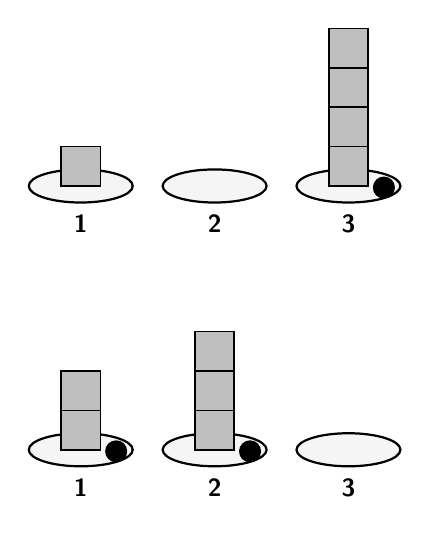
\begin{tikzpicture}[]
\draw[line width=0.8pt,fill=black!4] (0.000,3.350) ellipse (0.66 and 0.21);
\node[font=\small\bfseries] at (0.000,2.870) {1};
\draw[line width=0.6pt,fill=black!25] (-0.250,3.350) rectangle (0.250,3.850);
\draw[line width=0.8pt,fill=black!4] (1.700,3.350) ellipse (0.66 and 0.21);
\node[font=\small\bfseries] at (1.700,2.870) {2};
\draw[line width=0.8pt,fill=black!4] (3.400,3.350) ellipse (0.66 and 0.21);
\node[font=\small\bfseries] at (3.400,2.870) {3};
\draw[line width=0.6pt,fill=black!25] (3.150,3.350) rectangle (3.650,3.850);
\draw[line width=0.6pt,fill=black!25] (3.150,3.850) rectangle (3.650,4.350);
\draw[line width=0.6pt,fill=black!25] (3.150,4.350) rectangle (3.650,4.850);
\draw[line width=0.6pt,fill=black!25] (3.150,4.850) rectangle (3.650,5.350);
\fill (3.850,3.330) circle (0.14);
\draw[line width=0.8pt,fill=black!4] (0.000,0.000) ellipse (0.66 and 0.21);
\node[font=\small\bfseries] at (0.000,-0.480) {1};
\draw[line width=0.6pt,fill=black!25] (-0.250,0.000) rectangle (0.250,0.500);
\draw[line width=0.6pt,fill=black!25] (-0.250,0.500) rectangle (0.250,1.000);
\fill (0.450,-0.020) circle (0.14);
\draw[line width=0.8pt,fill=black!4] (1.700,0.000) ellipse (0.66 and 0.21);
\node[font=\small\bfseries] at (1.700,-0.480) {2};
\draw[line width=0.6pt,fill=black!25] (1.450,0.000) rectangle (1.950,0.500);
\draw[line width=0.6pt,fill=black!25] (1.450,0.500) rectangle (1.950,1.000);
\draw[line width=0.6pt,fill=black!25] (1.450,1.000) rectangle (1.950,1.500);
\fill (2.150,-0.020) circle (0.14);
\draw[line width=0.8pt,fill=black!4] (3.400,0.000) ellipse (0.66 and 0.21);
\node[font=\small\bfseries] at (3.400,-0.480) {3};
\end{tikzpicture}\end{minipage}
\prob{1}Play with 5 cubes each. In each new game, try to beat the plan your partner just used.
\prob{2}Your partner can see your plan and tries to beat it. Is there a plan with 5 cubes that nobody can beat?
\par\vspace{10pt}\noindent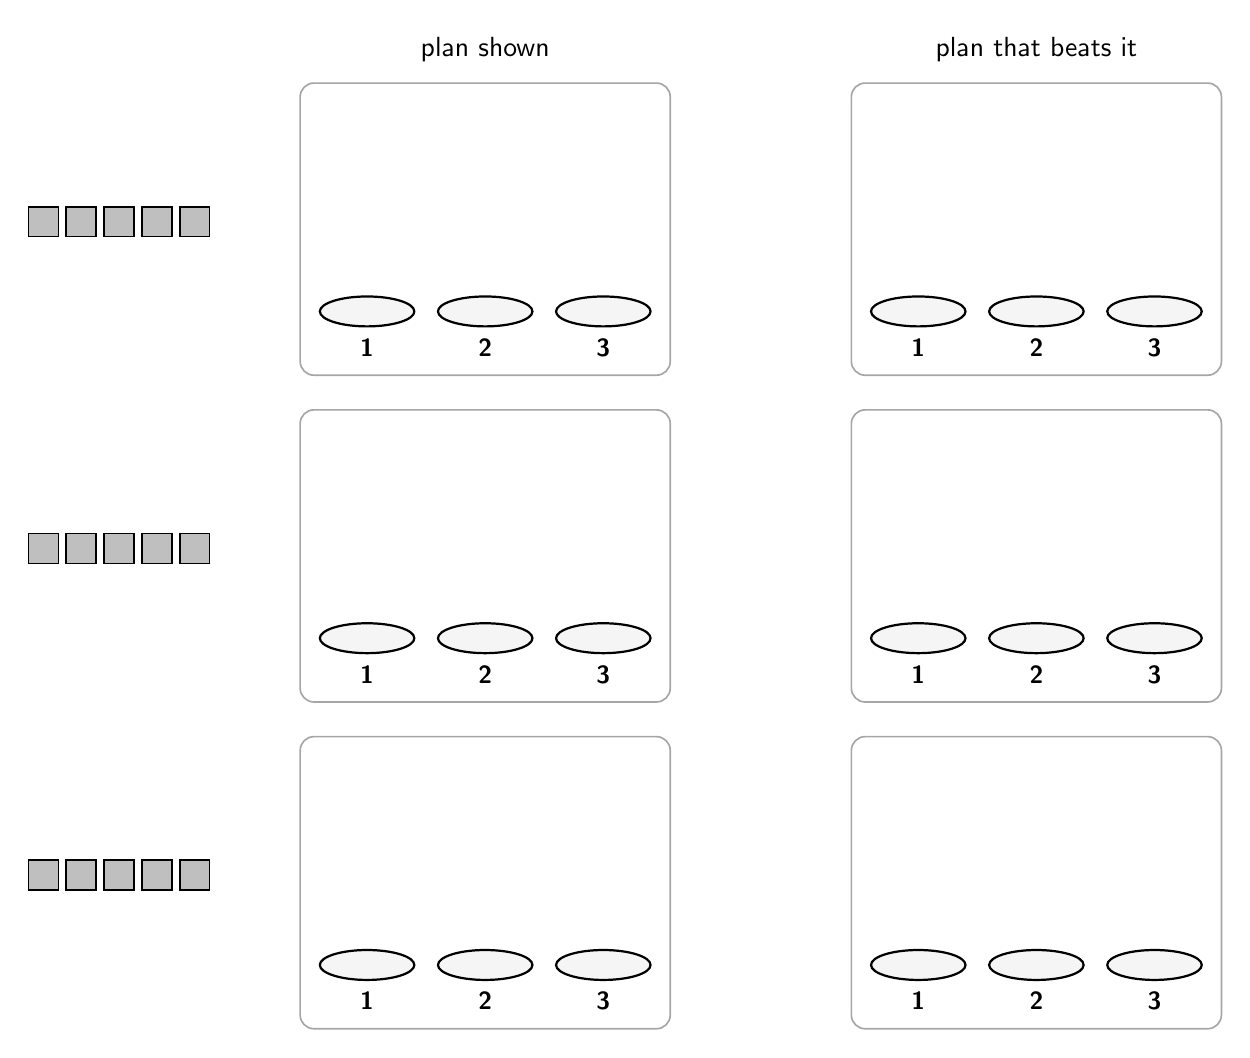
\begin{tikzpicture}[]
\node[font=\normalsize,anchor=south] at (5.800,3.05) {plan shown};
\node[font=\normalsize,anchor=south] at (12.800,3.05) {plan that beats it};
\draw[line width=0.6pt,fill=black!25] (0.000,0.950) rectangle (0.380,1.330);
\draw[line width=0.6pt,fill=black!25] (0.480,0.950) rectangle (0.860,1.330);
\draw[line width=0.6pt,fill=black!25] (0.960,0.950) rectangle (1.340,1.330);
\draw[line width=0.6pt,fill=black!25] (1.440,0.950) rectangle (1.820,1.330);
\draw[line width=0.6pt,fill=black!25] (1.920,0.950) rectangle (2.300,1.330);
\draw[black!35,line width=0.6pt,rounded corners=5pt] (3.450,-0.810) rectangle (8.150,2.900);
\draw[line width=0.8pt,fill=black!4] (4.300,0.000) ellipse (0.6 and 0.19);
\node[font=\small\bfseries] at (4.300,-0.460) {1};
\draw[line width=0.8pt,fill=black!4] (5.800,0.000) ellipse (0.6 and 0.19);
\node[font=\small\bfseries] at (5.800,-0.460) {2};
\draw[line width=0.8pt,fill=black!4] (7.300,0.000) ellipse (0.6 and 0.19);
\node[font=\small\bfseries] at (7.300,-0.460) {3};
\draw[black!35,line width=0.6pt,rounded corners=5pt] (10.450,-0.810) rectangle (15.150,2.900);
\draw[line width=0.8pt,fill=black!4] (11.300,0.000) ellipse (0.6 and 0.19);
\node[font=\small\bfseries] at (11.300,-0.460) {1};
\draw[line width=0.8pt,fill=black!4] (12.800,0.000) ellipse (0.6 and 0.19);
\node[font=\small\bfseries] at (12.800,-0.460) {2};
\draw[line width=0.8pt,fill=black!4] (14.300,0.000) ellipse (0.6 and 0.19);
\node[font=\small\bfseries] at (14.300,-0.460) {3};
\draw[line width=0.6pt,fill=black!25] (0.000,-3.200) rectangle (0.380,-2.820);
\draw[line width=0.6pt,fill=black!25] (0.480,-3.200) rectangle (0.860,-2.820);
\draw[line width=0.6pt,fill=black!25] (0.960,-3.200) rectangle (1.340,-2.820);
\draw[line width=0.6pt,fill=black!25] (1.440,-3.200) rectangle (1.820,-2.820);
\draw[line width=0.6pt,fill=black!25] (1.920,-3.200) rectangle (2.300,-2.820);
\draw[black!35,line width=0.6pt,rounded corners=5pt] (3.450,-4.960) rectangle (8.150,-1.250);
\draw[line width=0.8pt,fill=black!4] (4.300,-4.150) ellipse (0.6 and 0.19);
\node[font=\small\bfseries] at (4.300,-4.610) {1};
\draw[line width=0.8pt,fill=black!4] (5.800,-4.150) ellipse (0.6 and 0.19);
\node[font=\small\bfseries] at (5.800,-4.610) {2};
\draw[line width=0.8pt,fill=black!4] (7.300,-4.150) ellipse (0.6 and 0.19);
\node[font=\small\bfseries] at (7.300,-4.610) {3};
\draw[black!35,line width=0.6pt,rounded corners=5pt] (10.450,-4.960) rectangle (15.150,-1.250);
\draw[line width=0.8pt,fill=black!4] (11.300,-4.150) ellipse (0.6 and 0.19);
\node[font=\small\bfseries] at (11.300,-4.610) {1};
\draw[line width=0.8pt,fill=black!4] (12.800,-4.150) ellipse (0.6 and 0.19);
\node[font=\small\bfseries] at (12.800,-4.610) {2};
\draw[line width=0.8pt,fill=black!4] (14.300,-4.150) ellipse (0.6 and 0.19);
\node[font=\small\bfseries] at (14.300,-4.610) {3};
\draw[line width=0.6pt,fill=black!25] (0.000,-7.350) rectangle (0.380,-6.970);
\draw[line width=0.6pt,fill=black!25] (0.480,-7.350) rectangle (0.860,-6.970);
\draw[line width=0.6pt,fill=black!25] (0.960,-7.350) rectangle (1.340,-6.970);
\draw[line width=0.6pt,fill=black!25] (1.440,-7.350) rectangle (1.820,-6.970);
\draw[line width=0.6pt,fill=black!25] (1.920,-7.350) rectangle (2.300,-6.970);
\draw[black!35,line width=0.6pt,rounded corners=5pt] (3.450,-9.110) rectangle (8.150,-5.400);
\draw[line width=0.8pt,fill=black!4] (4.300,-8.300) ellipse (0.6 and 0.19);
\node[font=\small\bfseries] at (4.300,-8.760) {1};
\draw[line width=0.8pt,fill=black!4] (5.800,-8.300) ellipse (0.6 and 0.19);
\node[font=\small\bfseries] at (5.800,-8.760) {2};
\draw[line width=0.8pt,fill=black!4] (7.300,-8.300) ellipse (0.6 and 0.19);
\node[font=\small\bfseries] at (7.300,-8.760) {3};
\draw[black!35,line width=0.6pt,rounded corners=5pt] (10.450,-9.110) rectangle (15.150,-5.400);
\draw[line width=0.8pt,fill=black!4] (11.300,-8.300) ellipse (0.6 and 0.19);
\node[font=\small\bfseries] at (11.300,-8.760) {1};
\draw[line width=0.8pt,fill=black!4] (12.800,-8.300) ellipse (0.6 and 0.19);
\node[font=\small\bfseries] at (12.800,-8.760) {2};
\draw[line width=0.8pt,fill=black!4] (14.300,-8.300) ellipse (0.6 and 0.19);
\node[font=\small\bfseries] at (14.300,-8.760) {3};
\end{tikzpicture}
\newpage
\prob{3}For each plan below, draw a plan with 5 cubes that beats it.
\par\vspace{12pt}\noindent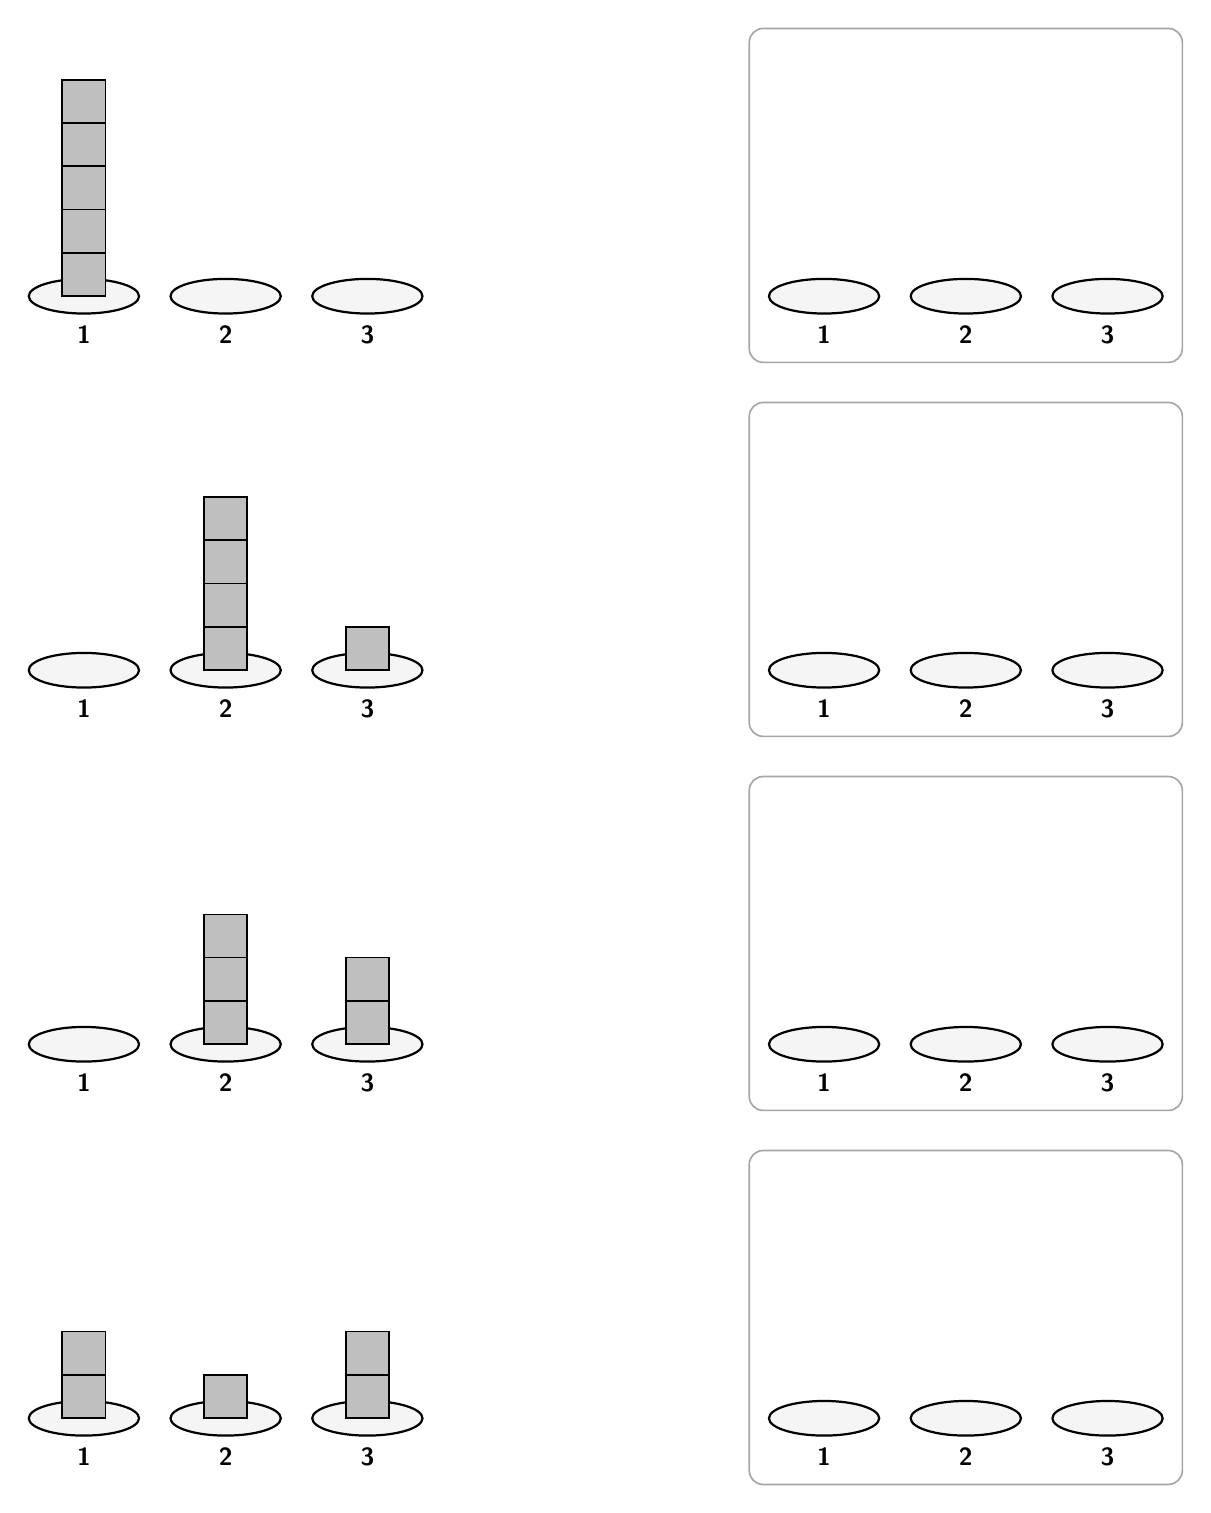
\begin{tikzpicture}[]
\draw[line width=0.8pt,fill=black!4] (1.200,0.000) ellipse (0.7 and 0.22);
\node[font=\small\bfseries] at (1.200,-0.490) {1};
\draw[line width=0.6pt,fill=black!25] (0.925,0.000) rectangle (1.475,0.550);
\draw[line width=0.6pt,fill=black!25] (0.925,0.550) rectangle (1.475,1.100);
\draw[line width=0.6pt,fill=black!25] (0.925,1.100) rectangle (1.475,1.650);
\draw[line width=0.6pt,fill=black!25] (0.925,1.650) rectangle (1.475,2.200);
\draw[line width=0.6pt,fill=black!25] (0.925,2.200) rectangle (1.475,2.750);
\draw[line width=0.8pt,fill=black!4] (3.000,0.000) ellipse (0.7 and 0.22);
\node[font=\small\bfseries] at (3.000,-0.490) {2};
\draw[line width=0.8pt,fill=black!4] (4.800,0.000) ellipse (0.7 and 0.22);
\node[font=\small\bfseries] at (4.800,-0.490) {3};
\draw[black!35,line width=0.6pt,rounded corners=5pt] (9.650,-0.840) rectangle (15.150,3.400);
\draw[line width=0.8pt,fill=black!4] (10.600,0.000) ellipse (0.7 and 0.22);
\node[font=\small\bfseries] at (10.600,-0.490) {1};
\draw[line width=0.8pt,fill=black!4] (12.400,0.000) ellipse (0.7 and 0.22);
\node[font=\small\bfseries] at (12.400,-0.490) {2};
\draw[line width=0.8pt,fill=black!4] (14.200,0.000) ellipse (0.7 and 0.22);
\node[font=\small\bfseries] at (14.200,-0.490) {3};
\draw[line width=0.8pt,fill=black!4] (1.200,-4.750) ellipse (0.7 and 0.22);
\node[font=\small\bfseries] at (1.200,-5.240) {1};
\draw[line width=0.8pt,fill=black!4] (3.000,-4.750) ellipse (0.7 and 0.22);
\node[font=\small\bfseries] at (3.000,-5.240) {2};
\draw[line width=0.6pt,fill=black!25] (2.725,-4.750) rectangle (3.275,-4.200);
\draw[line width=0.6pt,fill=black!25] (2.725,-4.200) rectangle (3.275,-3.650);
\draw[line width=0.6pt,fill=black!25] (2.725,-3.650) rectangle (3.275,-3.100);
\draw[line width=0.6pt,fill=black!25] (2.725,-3.100) rectangle (3.275,-2.550);
\draw[line width=0.8pt,fill=black!4] (4.800,-4.750) ellipse (0.7 and 0.22);
\node[font=\small\bfseries] at (4.800,-5.240) {3};
\draw[line width=0.6pt,fill=black!25] (4.525,-4.750) rectangle (5.075,-4.200);
\draw[black!35,line width=0.6pt,rounded corners=5pt] (9.650,-5.590) rectangle (15.150,-1.350);
\draw[line width=0.8pt,fill=black!4] (10.600,-4.750) ellipse (0.7 and 0.22);
\node[font=\small\bfseries] at (10.600,-5.240) {1};
\draw[line width=0.8pt,fill=black!4] (12.400,-4.750) ellipse (0.7 and 0.22);
\node[font=\small\bfseries] at (12.400,-5.240) {2};
\draw[line width=0.8pt,fill=black!4] (14.200,-4.750) ellipse (0.7 and 0.22);
\node[font=\small\bfseries] at (14.200,-5.240) {3};
\draw[line width=0.8pt,fill=black!4] (1.200,-9.500) ellipse (0.7 and 0.22);
\node[font=\small\bfseries] at (1.200,-9.990) {1};
\draw[line width=0.8pt,fill=black!4] (3.000,-9.500) ellipse (0.7 and 0.22);
\node[font=\small\bfseries] at (3.000,-9.990) {2};
\draw[line width=0.6pt,fill=black!25] (2.725,-9.500) rectangle (3.275,-8.950);
\draw[line width=0.6pt,fill=black!25] (2.725,-8.950) rectangle (3.275,-8.400);
\draw[line width=0.6pt,fill=black!25] (2.725,-8.400) rectangle (3.275,-7.850);
\draw[line width=0.8pt,fill=black!4] (4.800,-9.500) ellipse (0.7 and 0.22);
\node[font=\small\bfseries] at (4.800,-9.990) {3};
\draw[line width=0.6pt,fill=black!25] (4.525,-9.500) rectangle (5.075,-8.950);
\draw[line width=0.6pt,fill=black!25] (4.525,-8.950) rectangle (5.075,-8.400);
\draw[black!35,line width=0.6pt,rounded corners=5pt] (9.650,-10.340) rectangle (15.150,-6.100);
\draw[line width=0.8pt,fill=black!4] (10.600,-9.500) ellipse (0.7 and 0.22);
\node[font=\small\bfseries] at (10.600,-9.990) {1};
\draw[line width=0.8pt,fill=black!4] (12.400,-9.500) ellipse (0.7 and 0.22);
\node[font=\small\bfseries] at (12.400,-9.990) {2};
\draw[line width=0.8pt,fill=black!4] (14.200,-9.500) ellipse (0.7 and 0.22);
\node[font=\small\bfseries] at (14.200,-9.990) {3};
\draw[line width=0.8pt,fill=black!4] (1.200,-14.250) ellipse (0.7 and 0.22);
\node[font=\small\bfseries] at (1.200,-14.740) {1};
\draw[line width=0.6pt,fill=black!25] (0.925,-14.250) rectangle (1.475,-13.700);
\draw[line width=0.6pt,fill=black!25] (0.925,-13.700) rectangle (1.475,-13.150);
\draw[line width=0.8pt,fill=black!4] (3.000,-14.250) ellipse (0.7 and 0.22);
\node[font=\small\bfseries] at (3.000,-14.740) {2};
\draw[line width=0.6pt,fill=black!25] (2.725,-14.250) rectangle (3.275,-13.700);
\draw[line width=0.8pt,fill=black!4] (4.800,-14.250) ellipse (0.7 and 0.22);
\node[font=\small\bfseries] at (4.800,-14.740) {3};
\draw[line width=0.6pt,fill=black!25] (4.525,-14.250) rectangle (5.075,-13.700);
\draw[line width=0.6pt,fill=black!25] (4.525,-13.700) rectangle (5.075,-13.150);
\draw[black!35,line width=0.6pt,rounded corners=5pt] (9.650,-15.090) rectangle (15.150,-10.850);
\draw[line width=0.8pt,fill=black!4] (10.600,-14.250) ellipse (0.7 and 0.22);
\node[font=\small\bfseries] at (10.600,-14.740) {1};
\draw[line width=0.8pt,fill=black!4] (12.400,-14.250) ellipse (0.7 and 0.22);
\node[font=\small\bfseries] at (12.400,-14.740) {2};
\draw[line width=0.8pt,fill=black!4] (14.200,-14.250) ellipse (0.7 and 0.22);
\node[font=\small\bfseries] at (14.200,-14.740) {3};
\end{tikzpicture}
\newpage
\prob{4}Is there a plan that nobody can beat when each player has 2 cubes? 3 cubes? 4 cubes?
\par\vspace{12pt}\noindent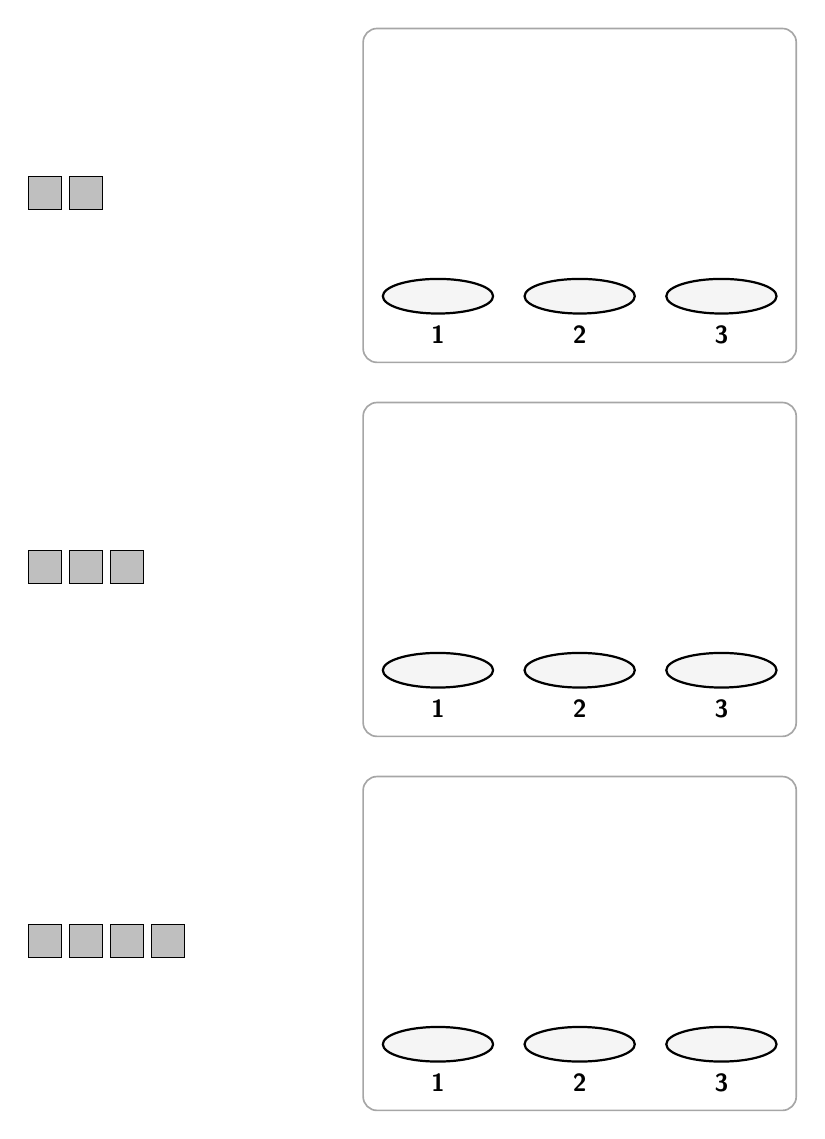
\begin{tikzpicture}[]
\draw[line width=0.6pt,fill=black!25] (1.000,1.100) rectangle (1.420,1.520);
\draw[line width=0.6pt,fill=black!25] (1.520,1.100) rectangle (1.940,1.520);
\draw[black!35,line width=0.6pt,rounded corners=5pt] (5.250,-0.840) rectangle (10.750,3.400);
\draw[line width=0.8pt,fill=black!4] (6.200,0.000) ellipse (0.7 and 0.22);
\node[font=\small\bfseries] at (6.200,-0.490) {1};
\draw[line width=0.8pt,fill=black!4] (8.000,0.000) ellipse (0.7 and 0.22);
\node[font=\small\bfseries] at (8.000,-0.490) {2};
\draw[line width=0.8pt,fill=black!4] (9.800,0.000) ellipse (0.7 and 0.22);
\node[font=\small\bfseries] at (9.800,-0.490) {3};
\draw[line width=0.6pt,fill=black!25] (1.000,-3.650) rectangle (1.420,-3.230);
\draw[line width=0.6pt,fill=black!25] (1.520,-3.650) rectangle (1.940,-3.230);
\draw[line width=0.6pt,fill=black!25] (2.040,-3.650) rectangle (2.460,-3.230);
\draw[black!35,line width=0.6pt,rounded corners=5pt] (5.250,-5.590) rectangle (10.750,-1.350);
\draw[line width=0.8pt,fill=black!4] (6.200,-4.750) ellipse (0.7 and 0.22);
\node[font=\small\bfseries] at (6.200,-5.240) {1};
\draw[line width=0.8pt,fill=black!4] (8.000,-4.750) ellipse (0.7 and 0.22);
\node[font=\small\bfseries] at (8.000,-5.240) {2};
\draw[line width=0.8pt,fill=black!4] (9.800,-4.750) ellipse (0.7 and 0.22);
\node[font=\small\bfseries] at (9.800,-5.240) {3};
\draw[line width=0.6pt,fill=black!25] (1.000,-8.400) rectangle (1.420,-7.980);
\draw[line width=0.6pt,fill=black!25] (1.520,-8.400) rectangle (1.940,-7.980);
\draw[line width=0.6pt,fill=black!25] (2.040,-8.400) rectangle (2.460,-7.980);
\draw[line width=0.6pt,fill=black!25] (2.560,-8.400) rectangle (2.980,-7.980);
\draw[black!35,line width=0.6pt,rounded corners=5pt] (5.250,-10.340) rectangle (10.750,-6.100);
\draw[line width=0.8pt,fill=black!4] (6.200,-9.500) ellipse (0.7 and 0.22);
\node[font=\small\bfseries] at (6.200,-9.990) {1};
\draw[line width=0.8pt,fill=black!4] (8.000,-9.500) ellipse (0.7 and 0.22);
\node[font=\small\bfseries] at (8.000,-9.990) {2};
\draw[line width=0.8pt,fill=black!4] (9.800,-9.500) ellipse (0.7 and 0.22);
\node[font=\small\bfseries] at (9.800,-9.990) {3};
\end{tikzpicture}
\newpage
\prob{5}Build the two plans in each row and circle the winner. In each box, is one plan the best?
\par\vspace{12pt}\noindent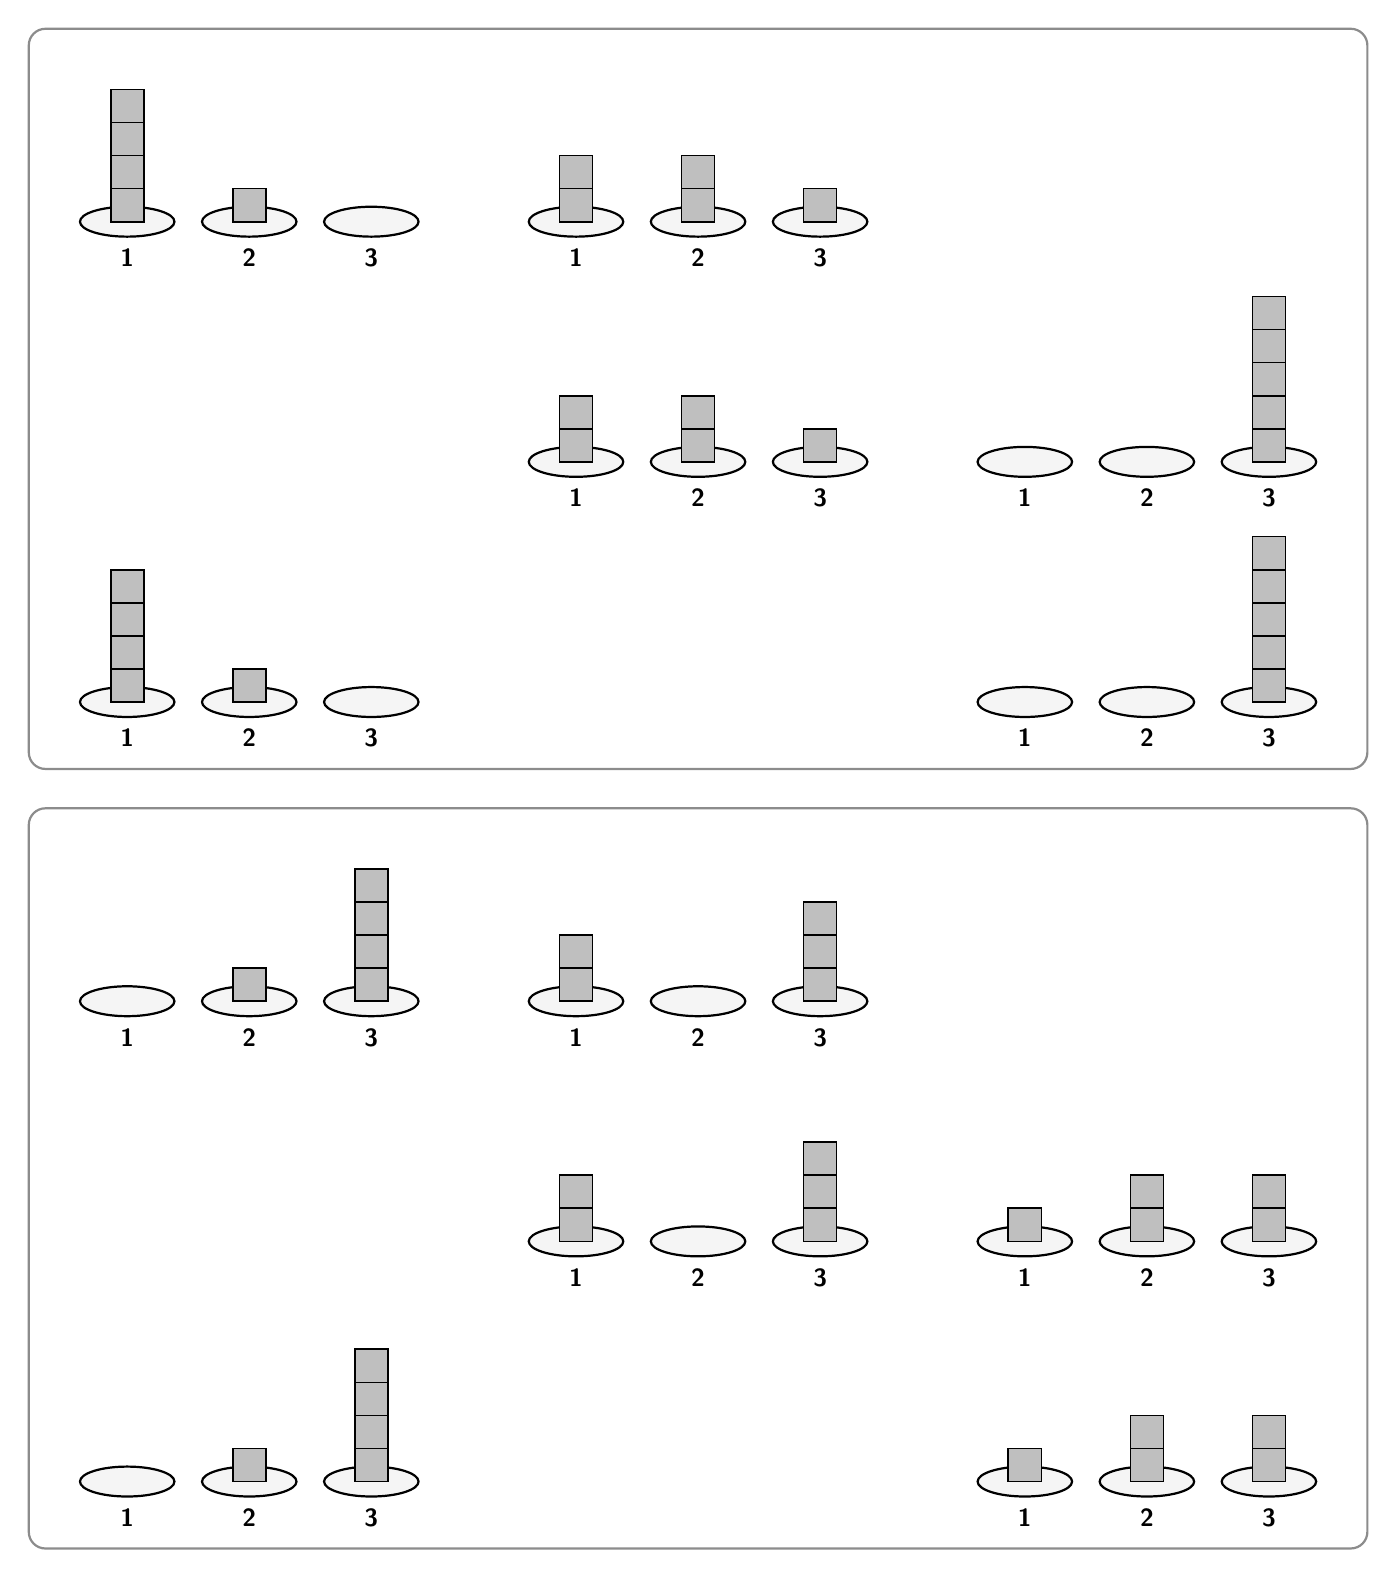
\begin{tikzpicture}[]
\draw[line width=0.8pt,fill=black!4] (1.550,0.000) ellipse (0.6 and 0.19);
\node[font=\small\bfseries] at (1.550,-0.460) {1};
\draw[line width=0.6pt,fill=black!25] (1.340,0.000) rectangle (1.760,0.420);
\draw[line width=0.6pt,fill=black!25] (1.340,0.420) rectangle (1.760,0.840);
\draw[line width=0.6pt,fill=black!25] (1.340,0.840) rectangle (1.760,1.260);
\draw[line width=0.6pt,fill=black!25] (1.340,1.260) rectangle (1.760,1.680);
\draw[line width=0.8pt,fill=black!4] (3.100,0.000) ellipse (0.6 and 0.19);
\node[font=\small\bfseries] at (3.100,-0.460) {2};
\draw[line width=0.6pt,fill=black!25] (2.890,0.000) rectangle (3.310,0.420);
\draw[line width=0.8pt,fill=black!4] (4.650,0.000) ellipse (0.6 and 0.19);
\node[font=\small\bfseries] at (4.650,-0.460) {3};
\draw[line width=0.8pt,fill=black!4] (7.250,0.000) ellipse (0.6 and 0.19);
\node[font=\small\bfseries] at (7.250,-0.460) {1};
\draw[line width=0.6pt,fill=black!25] (7.040,0.000) rectangle (7.460,0.420);
\draw[line width=0.6pt,fill=black!25] (7.040,0.420) rectangle (7.460,0.840);
\draw[line width=0.8pt,fill=black!4] (8.800,0.000) ellipse (0.6 and 0.19);
\node[font=\small\bfseries] at (8.800,-0.460) {2};
\draw[line width=0.6pt,fill=black!25] (8.590,0.000) rectangle (9.010,0.420);
\draw[line width=0.6pt,fill=black!25] (8.590,0.420) rectangle (9.010,0.840);
\draw[line width=0.8pt,fill=black!4] (10.350,0.000) ellipse (0.6 and 0.19);
\node[font=\small\bfseries] at (10.350,-0.460) {3};
\draw[line width=0.6pt,fill=black!25] (10.140,0.000) rectangle (10.560,0.420);
\draw[line width=0.8pt,fill=black!4] (7.250,-3.050) ellipse (0.6 and 0.19);
\node[font=\small\bfseries] at (7.250,-3.510) {1};
\draw[line width=0.6pt,fill=black!25] (7.040,-3.050) rectangle (7.460,-2.630);
\draw[line width=0.6pt,fill=black!25] (7.040,-2.630) rectangle (7.460,-2.210);
\draw[line width=0.8pt,fill=black!4] (8.800,-3.050) ellipse (0.6 and 0.19);
\node[font=\small\bfseries] at (8.800,-3.510) {2};
\draw[line width=0.6pt,fill=black!25] (8.590,-3.050) rectangle (9.010,-2.630);
\draw[line width=0.6pt,fill=black!25] (8.590,-2.630) rectangle (9.010,-2.210);
\draw[line width=0.8pt,fill=black!4] (10.350,-3.050) ellipse (0.6 and 0.19);
\node[font=\small\bfseries] at (10.350,-3.510) {3};
\draw[line width=0.6pt,fill=black!25] (10.140,-3.050) rectangle (10.560,-2.630);
\draw[line width=0.8pt,fill=black!4] (12.950,-3.050) ellipse (0.6 and 0.19);
\node[font=\small\bfseries] at (12.950,-3.510) {1};
\draw[line width=0.8pt,fill=black!4] (14.500,-3.050) ellipse (0.6 and 0.19);
\node[font=\small\bfseries] at (14.500,-3.510) {2};
\draw[line width=0.8pt,fill=black!4] (16.050,-3.050) ellipse (0.6 and 0.19);
\node[font=\small\bfseries] at (16.050,-3.510) {3};
\draw[line width=0.6pt,fill=black!25] (15.840,-3.050) rectangle (16.260,-2.630);
\draw[line width=0.6pt,fill=black!25] (15.840,-2.630) rectangle (16.260,-2.210);
\draw[line width=0.6pt,fill=black!25] (15.840,-2.210) rectangle (16.260,-1.790);
\draw[line width=0.6pt,fill=black!25] (15.840,-1.790) rectangle (16.260,-1.370);
\draw[line width=0.6pt,fill=black!25] (15.840,-1.370) rectangle (16.260,-0.950);
\draw[line width=0.8pt,fill=black!4] (1.550,-6.100) ellipse (0.6 and 0.19);
\node[font=\small\bfseries] at (1.550,-6.560) {1};
\draw[line width=0.6pt,fill=black!25] (1.340,-6.100) rectangle (1.760,-5.680);
\draw[line width=0.6pt,fill=black!25] (1.340,-5.680) rectangle (1.760,-5.260);
\draw[line width=0.6pt,fill=black!25] (1.340,-5.260) rectangle (1.760,-4.840);
\draw[line width=0.6pt,fill=black!25] (1.340,-4.840) rectangle (1.760,-4.420);
\draw[line width=0.8pt,fill=black!4] (3.100,-6.100) ellipse (0.6 and 0.19);
\node[font=\small\bfseries] at (3.100,-6.560) {2};
\draw[line width=0.6pt,fill=black!25] (2.890,-6.100) rectangle (3.310,-5.680);
\draw[line width=0.8pt,fill=black!4] (4.650,-6.100) ellipse (0.6 and 0.19);
\node[font=\small\bfseries] at (4.650,-6.560) {3};
\draw[line width=0.8pt,fill=black!4] (12.950,-6.100) ellipse (0.6 and 0.19);
\node[font=\small\bfseries] at (12.950,-6.560) {1};
\draw[line width=0.8pt,fill=black!4] (14.500,-6.100) ellipse (0.6 and 0.19);
\node[font=\small\bfseries] at (14.500,-6.560) {2};
\draw[line width=0.8pt,fill=black!4] (16.050,-6.100) ellipse (0.6 and 0.19);
\node[font=\small\bfseries] at (16.050,-6.560) {3};
\draw[line width=0.6pt,fill=black!25] (15.840,-6.100) rectangle (16.260,-5.680);
\draw[line width=0.6pt,fill=black!25] (15.840,-5.680) rectangle (16.260,-5.260);
\draw[line width=0.6pt,fill=black!25] (15.840,-5.260) rectangle (16.260,-4.840);
\draw[line width=0.6pt,fill=black!25] (15.840,-4.840) rectangle (16.260,-4.420);
\draw[line width=0.6pt,fill=black!25] (15.840,-4.420) rectangle (16.260,-4.000);
\draw[black!45,line width=0.8pt,rounded corners=6pt] (0.3,-6.950) rectangle (17.3,2.450);
\draw[line width=0.8pt,fill=black!4] (1.550,-9.900) ellipse (0.6 and 0.19);
\node[font=\small\bfseries] at (1.550,-10.360) {1};
\draw[line width=0.8pt,fill=black!4] (3.100,-9.900) ellipse (0.6 and 0.19);
\node[font=\small\bfseries] at (3.100,-10.360) {2};
\draw[line width=0.6pt,fill=black!25] (2.890,-9.900) rectangle (3.310,-9.480);
\draw[line width=0.8pt,fill=black!4] (4.650,-9.900) ellipse (0.6 and 0.19);
\node[font=\small\bfseries] at (4.650,-10.360) {3};
\draw[line width=0.6pt,fill=black!25] (4.440,-9.900) rectangle (4.860,-9.480);
\draw[line width=0.6pt,fill=black!25] (4.440,-9.480) rectangle (4.860,-9.060);
\draw[line width=0.6pt,fill=black!25] (4.440,-9.060) rectangle (4.860,-8.640);
\draw[line width=0.6pt,fill=black!25] (4.440,-8.640) rectangle (4.860,-8.220);
\draw[line width=0.8pt,fill=black!4] (7.250,-9.900) ellipse (0.6 and 0.19);
\node[font=\small\bfseries] at (7.250,-10.360) {1};
\draw[line width=0.6pt,fill=black!25] (7.040,-9.900) rectangle (7.460,-9.480);
\draw[line width=0.6pt,fill=black!25] (7.040,-9.480) rectangle (7.460,-9.060);
\draw[line width=0.8pt,fill=black!4] (8.800,-9.900) ellipse (0.6 and 0.19);
\node[font=\small\bfseries] at (8.800,-10.360) {2};
\draw[line width=0.8pt,fill=black!4] (10.350,-9.900) ellipse (0.6 and 0.19);
\node[font=\small\bfseries] at (10.350,-10.360) {3};
\draw[line width=0.6pt,fill=black!25] (10.140,-9.900) rectangle (10.560,-9.480);
\draw[line width=0.6pt,fill=black!25] (10.140,-9.480) rectangle (10.560,-9.060);
\draw[line width=0.6pt,fill=black!25] (10.140,-9.060) rectangle (10.560,-8.640);
\draw[line width=0.8pt,fill=black!4] (7.250,-12.950) ellipse (0.6 and 0.19);
\node[font=\small\bfseries] at (7.250,-13.410) {1};
\draw[line width=0.6pt,fill=black!25] (7.040,-12.950) rectangle (7.460,-12.530);
\draw[line width=0.6pt,fill=black!25] (7.040,-12.530) rectangle (7.460,-12.110);
\draw[line width=0.8pt,fill=black!4] (8.800,-12.950) ellipse (0.6 and 0.19);
\node[font=\small\bfseries] at (8.800,-13.410) {2};
\draw[line width=0.8pt,fill=black!4] (10.350,-12.950) ellipse (0.6 and 0.19);
\node[font=\small\bfseries] at (10.350,-13.410) {3};
\draw[line width=0.6pt,fill=black!25] (10.140,-12.950) rectangle (10.560,-12.530);
\draw[line width=0.6pt,fill=black!25] (10.140,-12.530) rectangle (10.560,-12.110);
\draw[line width=0.6pt,fill=black!25] (10.140,-12.110) rectangle (10.560,-11.690);
\draw[line width=0.8pt,fill=black!4] (12.950,-12.950) ellipse (0.6 and 0.19);
\node[font=\small\bfseries] at (12.950,-13.410) {1};
\draw[line width=0.6pt,fill=black!25] (12.740,-12.950) rectangle (13.160,-12.530);
\draw[line width=0.8pt,fill=black!4] (14.500,-12.950) ellipse (0.6 and 0.19);
\node[font=\small\bfseries] at (14.500,-13.410) {2};
\draw[line width=0.6pt,fill=black!25] (14.290,-12.950) rectangle (14.710,-12.530);
\draw[line width=0.6pt,fill=black!25] (14.290,-12.530) rectangle (14.710,-12.110);
\draw[line width=0.8pt,fill=black!4] (16.050,-12.950) ellipse (0.6 and 0.19);
\node[font=\small\bfseries] at (16.050,-13.410) {3};
\draw[line width=0.6pt,fill=black!25] (15.840,-12.950) rectangle (16.260,-12.530);
\draw[line width=0.6pt,fill=black!25] (15.840,-12.530) rectangle (16.260,-12.110);
\draw[line width=0.8pt,fill=black!4] (1.550,-16.000) ellipse (0.6 and 0.19);
\node[font=\small\bfseries] at (1.550,-16.460) {1};
\draw[line width=0.8pt,fill=black!4] (3.100,-16.000) ellipse (0.6 and 0.19);
\node[font=\small\bfseries] at (3.100,-16.460) {2};
\draw[line width=0.6pt,fill=black!25] (2.890,-16.000) rectangle (3.310,-15.580);
\draw[line width=0.8pt,fill=black!4] (4.650,-16.000) ellipse (0.6 and 0.19);
\node[font=\small\bfseries] at (4.650,-16.460) {3};
\draw[line width=0.6pt,fill=black!25] (4.440,-16.000) rectangle (4.860,-15.580);
\draw[line width=0.6pt,fill=black!25] (4.440,-15.580) rectangle (4.860,-15.160);
\draw[line width=0.6pt,fill=black!25] (4.440,-15.160) rectangle (4.860,-14.740);
\draw[line width=0.6pt,fill=black!25] (4.440,-14.740) rectangle (4.860,-14.320);
\draw[line width=0.8pt,fill=black!4] (12.950,-16.000) ellipse (0.6 and 0.19);
\node[font=\small\bfseries] at (12.950,-16.460) {1};
\draw[line width=0.6pt,fill=black!25] (12.740,-16.000) rectangle (13.160,-15.580);
\draw[line width=0.8pt,fill=black!4] (14.500,-16.000) ellipse (0.6 and 0.19);
\node[font=\small\bfseries] at (14.500,-16.460) {2};
\draw[line width=0.6pt,fill=black!25] (14.290,-16.000) rectangle (14.710,-15.580);
\draw[line width=0.6pt,fill=black!25] (14.290,-15.580) rectangle (14.710,-15.160);
\draw[line width=0.8pt,fill=black!4] (16.050,-16.000) ellipse (0.6 and 0.19);
\node[font=\small\bfseries] at (16.050,-16.460) {3};
\draw[line width=0.6pt,fill=black!25] (15.840,-16.000) rectangle (16.260,-15.580);
\draw[line width=0.6pt,fill=black!25] (15.840,-15.580) rectangle (16.260,-15.160);
\draw[black!45,line width=0.8pt,rounded corners=6pt] (0.3,-16.850) rectangle (17.3,-7.450);
\end{tikzpicture}
\newpage
\prob{6}You may use any number of cubes. For each plan below, draw a plan that beats it with as few cubes as you can.
\par\vspace{12pt}\noindent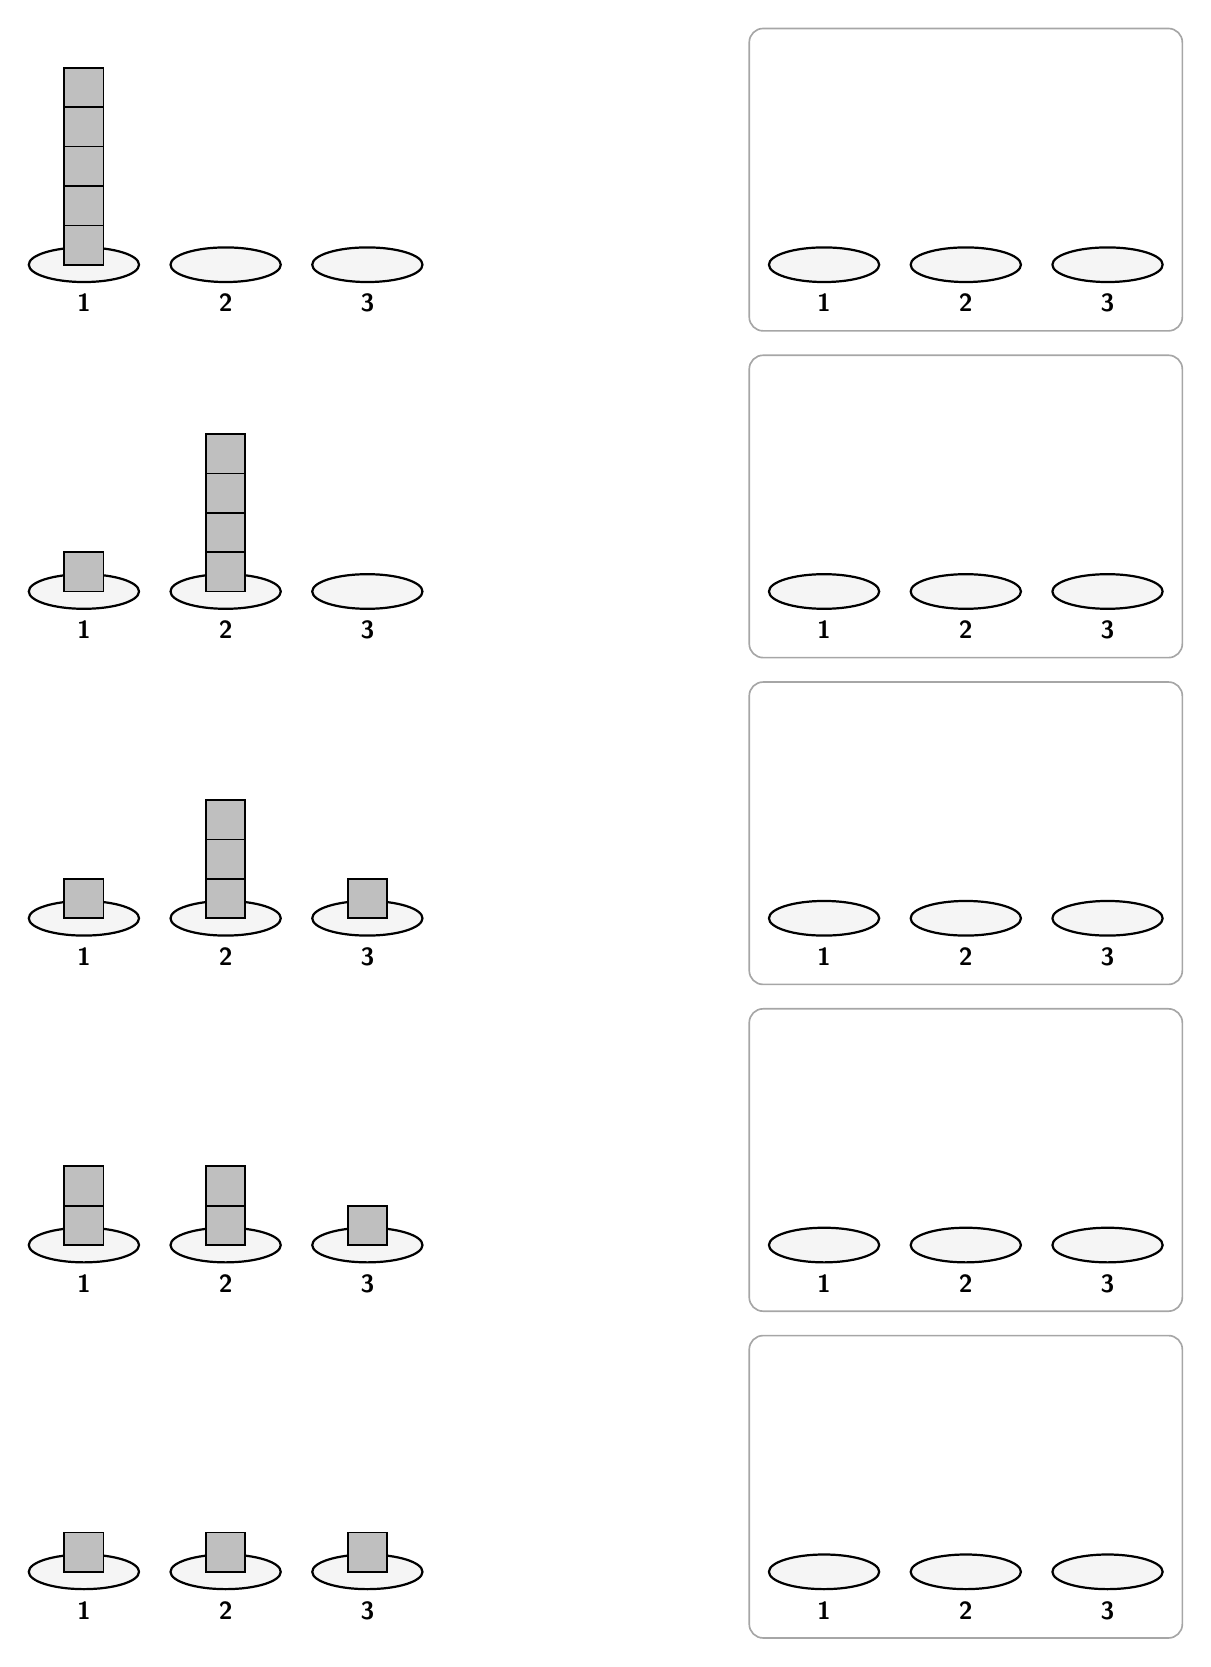
\begin{tikzpicture}[]
\draw[line width=0.8pt,fill=black!4] (1.200,0.000) ellipse (0.7 and 0.22);
\node[font=\small\bfseries] at (1.200,-0.490) {1};
\draw[line width=0.6pt,fill=black!25] (0.950,0.000) rectangle (1.450,0.500);
\draw[line width=0.6pt,fill=black!25] (0.950,0.500) rectangle (1.450,1.000);
\draw[line width=0.6pt,fill=black!25] (0.950,1.000) rectangle (1.450,1.500);
\draw[line width=0.6pt,fill=black!25] (0.950,1.500) rectangle (1.450,2.000);
\draw[line width=0.6pt,fill=black!25] (0.950,2.000) rectangle (1.450,2.500);
\draw[line width=0.8pt,fill=black!4] (3.000,0.000) ellipse (0.7 and 0.22);
\node[font=\small\bfseries] at (3.000,-0.490) {2};
\draw[line width=0.8pt,fill=black!4] (4.800,0.000) ellipse (0.7 and 0.22);
\node[font=\small\bfseries] at (4.800,-0.490) {3};
\draw[black!35,line width=0.6pt,rounded corners=5pt] (9.650,-0.840) rectangle (15.150,3.000);
\draw[line width=0.8pt,fill=black!4] (10.600,0.000) ellipse (0.7 and 0.22);
\node[font=\small\bfseries] at (10.600,-0.490) {1};
\draw[line width=0.8pt,fill=black!4] (12.400,0.000) ellipse (0.7 and 0.22);
\node[font=\small\bfseries] at (12.400,-0.490) {2};
\draw[line width=0.8pt,fill=black!4] (14.200,0.000) ellipse (0.7 and 0.22);
\node[font=\small\bfseries] at (14.200,-0.490) {3};
\draw[line width=0.8pt,fill=black!4] (1.200,-4.150) ellipse (0.7 and 0.22);
\node[font=\small\bfseries] at (1.200,-4.640) {1};
\draw[line width=0.6pt,fill=black!25] (0.950,-4.150) rectangle (1.450,-3.650);
\draw[line width=0.8pt,fill=black!4] (3.000,-4.150) ellipse (0.7 and 0.22);
\node[font=\small\bfseries] at (3.000,-4.640) {2};
\draw[line width=0.6pt,fill=black!25] (2.750,-4.150) rectangle (3.250,-3.650);
\draw[line width=0.6pt,fill=black!25] (2.750,-3.650) rectangle (3.250,-3.150);
\draw[line width=0.6pt,fill=black!25] (2.750,-3.150) rectangle (3.250,-2.650);
\draw[line width=0.6pt,fill=black!25] (2.750,-2.650) rectangle (3.250,-2.150);
\draw[line width=0.8pt,fill=black!4] (4.800,-4.150) ellipse (0.7 and 0.22);
\node[font=\small\bfseries] at (4.800,-4.640) {3};
\draw[black!35,line width=0.6pt,rounded corners=5pt] (9.650,-4.990) rectangle (15.150,-1.150);
\draw[line width=0.8pt,fill=black!4] (10.600,-4.150) ellipse (0.7 and 0.22);
\node[font=\small\bfseries] at (10.600,-4.640) {1};
\draw[line width=0.8pt,fill=black!4] (12.400,-4.150) ellipse (0.7 and 0.22);
\node[font=\small\bfseries] at (12.400,-4.640) {2};
\draw[line width=0.8pt,fill=black!4] (14.200,-4.150) ellipse (0.7 and 0.22);
\node[font=\small\bfseries] at (14.200,-4.640) {3};
\draw[line width=0.8pt,fill=black!4] (1.200,-8.300) ellipse (0.7 and 0.22);
\node[font=\small\bfseries] at (1.200,-8.790) {1};
\draw[line width=0.6pt,fill=black!25] (0.950,-8.300) rectangle (1.450,-7.800);
\draw[line width=0.8pt,fill=black!4] (3.000,-8.300) ellipse (0.7 and 0.22);
\node[font=\small\bfseries] at (3.000,-8.790) {2};
\draw[line width=0.6pt,fill=black!25] (2.750,-8.300) rectangle (3.250,-7.800);
\draw[line width=0.6pt,fill=black!25] (2.750,-7.800) rectangle (3.250,-7.300);
\draw[line width=0.6pt,fill=black!25] (2.750,-7.300) rectangle (3.250,-6.800);
\draw[line width=0.8pt,fill=black!4] (4.800,-8.300) ellipse (0.7 and 0.22);
\node[font=\small\bfseries] at (4.800,-8.790) {3};
\draw[line width=0.6pt,fill=black!25] (4.550,-8.300) rectangle (5.050,-7.800);
\draw[black!35,line width=0.6pt,rounded corners=5pt] (9.650,-9.140) rectangle (15.150,-5.300);
\draw[line width=0.8pt,fill=black!4] (10.600,-8.300) ellipse (0.7 and 0.22);
\node[font=\small\bfseries] at (10.600,-8.790) {1};
\draw[line width=0.8pt,fill=black!4] (12.400,-8.300) ellipse (0.7 and 0.22);
\node[font=\small\bfseries] at (12.400,-8.790) {2};
\draw[line width=0.8pt,fill=black!4] (14.200,-8.300) ellipse (0.7 and 0.22);
\node[font=\small\bfseries] at (14.200,-8.790) {3};
\draw[line width=0.8pt,fill=black!4] (1.200,-12.450) ellipse (0.7 and 0.22);
\node[font=\small\bfseries] at (1.200,-12.940) {1};
\draw[line width=0.6pt,fill=black!25] (0.950,-12.450) rectangle (1.450,-11.950);
\draw[line width=0.6pt,fill=black!25] (0.950,-11.950) rectangle (1.450,-11.450);
\draw[line width=0.8pt,fill=black!4] (3.000,-12.450) ellipse (0.7 and 0.22);
\node[font=\small\bfseries] at (3.000,-12.940) {2};
\draw[line width=0.6pt,fill=black!25] (2.750,-12.450) rectangle (3.250,-11.950);
\draw[line width=0.6pt,fill=black!25] (2.750,-11.950) rectangle (3.250,-11.450);
\draw[line width=0.8pt,fill=black!4] (4.800,-12.450) ellipse (0.7 and 0.22);
\node[font=\small\bfseries] at (4.800,-12.940) {3};
\draw[line width=0.6pt,fill=black!25] (4.550,-12.450) rectangle (5.050,-11.950);
\draw[black!35,line width=0.6pt,rounded corners=5pt] (9.650,-13.290) rectangle (15.150,-9.450);
\draw[line width=0.8pt,fill=black!4] (10.600,-12.450) ellipse (0.7 and 0.22);
\node[font=\small\bfseries] at (10.600,-12.940) {1};
\draw[line width=0.8pt,fill=black!4] (12.400,-12.450) ellipse (0.7 and 0.22);
\node[font=\small\bfseries] at (12.400,-12.940) {2};
\draw[line width=0.8pt,fill=black!4] (14.200,-12.450) ellipse (0.7 and 0.22);
\node[font=\small\bfseries] at (14.200,-12.940) {3};
\draw[line width=0.8pt,fill=black!4] (1.200,-16.600) ellipse (0.7 and 0.22);
\node[font=\small\bfseries] at (1.200,-17.090) {1};
\draw[line width=0.6pt,fill=black!25] (0.950,-16.600) rectangle (1.450,-16.100);
\draw[line width=0.8pt,fill=black!4] (3.000,-16.600) ellipse (0.7 and 0.22);
\node[font=\small\bfseries] at (3.000,-17.090) {2};
\draw[line width=0.6pt,fill=black!25] (2.750,-16.600) rectangle (3.250,-16.100);
\draw[line width=0.8pt,fill=black!4] (4.800,-16.600) ellipse (0.7 and 0.22);
\node[font=\small\bfseries] at (4.800,-17.090) {3};
\draw[line width=0.6pt,fill=black!25] (4.550,-16.600) rectangle (5.050,-16.100);
\draw[black!35,line width=0.6pt,rounded corners=5pt] (9.650,-17.440) rectangle (15.150,-13.600);
\draw[line width=0.8pt,fill=black!4] (10.600,-16.600) ellipse (0.7 and 0.22);
\node[font=\small\bfseries] at (10.600,-17.090) {1};
\draw[line width=0.8pt,fill=black!4] (12.400,-16.600) ellipse (0.7 and 0.22);
\node[font=\small\bfseries] at (12.400,-17.090) {2};
\draw[line width=0.8pt,fill=black!4] (14.200,-16.600) ellipse (0.7 and 0.22);
\node[font=\small\bfseries] at (14.200,-17.090) {3};
\end{tikzpicture}
\newpage
\prob{7}For each plan below, find every plan with 5 cubes that beats it.
\par\vspace{12pt}\noindent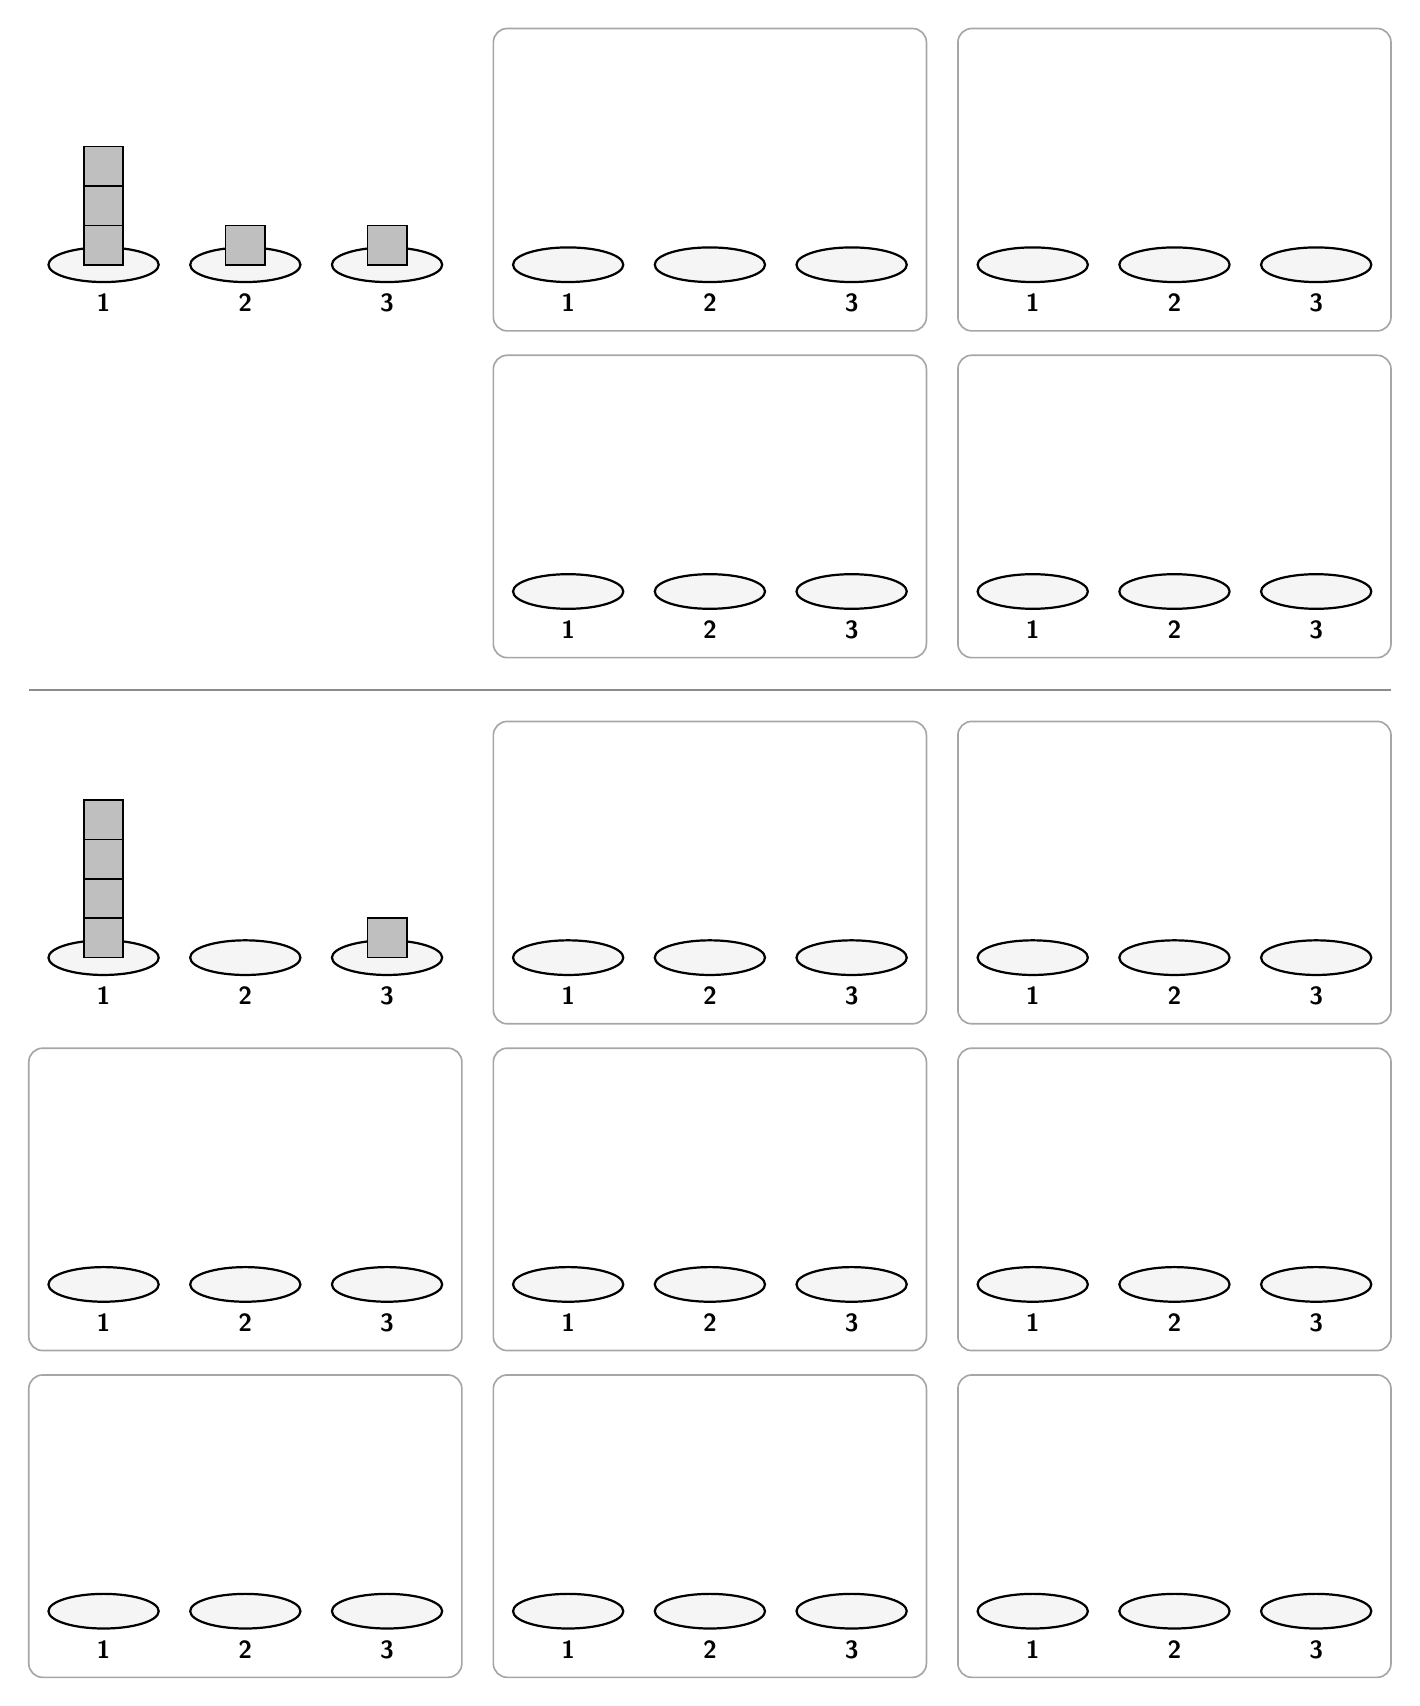
\begin{tikzpicture}[]
\draw[line width=0.8pt,fill=black!4] (0.950,0.000) ellipse (0.7 and 0.22);
\node[font=\small\bfseries] at (0.950,-0.490) {1};
\draw[line width=0.6pt,fill=black!25] (0.700,0.000) rectangle (1.200,0.500);
\draw[line width=0.6pt,fill=black!25] (0.700,0.500) rectangle (1.200,1.000);
\draw[line width=0.6pt,fill=black!25] (0.700,1.000) rectangle (1.200,1.500);
\draw[line width=0.8pt,fill=black!4] (2.750,0.000) ellipse (0.7 and 0.22);
\node[font=\small\bfseries] at (2.750,-0.490) {2};
\draw[line width=0.6pt,fill=black!25] (2.500,0.000) rectangle (3.000,0.500);
\draw[line width=0.8pt,fill=black!4] (4.550,0.000) ellipse (0.7 and 0.22);
\node[font=\small\bfseries] at (4.550,-0.490) {3};
\draw[line width=0.6pt,fill=black!25] (4.300,0.000) rectangle (4.800,0.500);
\draw[black!35,line width=0.6pt,rounded corners=5pt] (5.900,-0.840) rectangle (11.400,3.000);
\draw[line width=0.8pt,fill=black!4] (6.850,0.000) ellipse (0.7 and 0.22);
\node[font=\small\bfseries] at (6.850,-0.490) {1};
\draw[line width=0.8pt,fill=black!4] (8.650,0.000) ellipse (0.7 and 0.22);
\node[font=\small\bfseries] at (8.650,-0.490) {2};
\draw[line width=0.8pt,fill=black!4] (10.450,0.000) ellipse (0.7 and 0.22);
\node[font=\small\bfseries] at (10.450,-0.490) {3};
\draw[black!35,line width=0.6pt,rounded corners=5pt] (11.800,-0.840) rectangle (17.300,3.000);
\draw[line width=0.8pt,fill=black!4] (12.750,0.000) ellipse (0.7 and 0.22);
\node[font=\small\bfseries] at (12.750,-0.490) {1};
\draw[line width=0.8pt,fill=black!4] (14.550,0.000) ellipse (0.7 and 0.22);
\node[font=\small\bfseries] at (14.550,-0.490) {2};
\draw[line width=0.8pt,fill=black!4] (16.350,0.000) ellipse (0.7 and 0.22);
\node[font=\small\bfseries] at (16.350,-0.490) {3};
\draw[black!35,line width=0.6pt,rounded corners=5pt] (5.900,-4.990) rectangle (11.400,-1.150);
\draw[line width=0.8pt,fill=black!4] (6.850,-4.150) ellipse (0.7 and 0.22);
\node[font=\small\bfseries] at (6.850,-4.640) {1};
\draw[line width=0.8pt,fill=black!4] (8.650,-4.150) ellipse (0.7 and 0.22);
\node[font=\small\bfseries] at (8.650,-4.640) {2};
\draw[line width=0.8pt,fill=black!4] (10.450,-4.150) ellipse (0.7 and 0.22);
\node[font=\small\bfseries] at (10.450,-4.640) {3};
\draw[black!35,line width=0.6pt,rounded corners=5pt] (11.800,-4.990) rectangle (17.300,-1.150);
\draw[line width=0.8pt,fill=black!4] (12.750,-4.150) ellipse (0.7 and 0.22);
\node[font=\small\bfseries] at (12.750,-4.640) {1};
\draw[line width=0.8pt,fill=black!4] (14.550,-4.150) ellipse (0.7 and 0.22);
\node[font=\small\bfseries] at (14.550,-4.640) {2};
\draw[line width=0.8pt,fill=black!4] (16.350,-4.150) ellipse (0.7 and 0.22);
\node[font=\small\bfseries] at (16.350,-4.640) {3};
\draw[black!45,line width=0.8pt] (0,-5.400) -- (17.3,-5.400);
\draw[line width=0.8pt,fill=black!4] (0.950,-8.800) ellipse (0.7 and 0.22);
\node[font=\small\bfseries] at (0.950,-9.290) {1};
\draw[line width=0.6pt,fill=black!25] (0.700,-8.800) rectangle (1.200,-8.300);
\draw[line width=0.6pt,fill=black!25] (0.700,-8.300) rectangle (1.200,-7.800);
\draw[line width=0.6pt,fill=black!25] (0.700,-7.800) rectangle (1.200,-7.300);
\draw[line width=0.6pt,fill=black!25] (0.700,-7.300) rectangle (1.200,-6.800);
\draw[line width=0.8pt,fill=black!4] (2.750,-8.800) ellipse (0.7 and 0.22);
\node[font=\small\bfseries] at (2.750,-9.290) {2};
\draw[line width=0.8pt,fill=black!4] (4.550,-8.800) ellipse (0.7 and 0.22);
\node[font=\small\bfseries] at (4.550,-9.290) {3};
\draw[line width=0.6pt,fill=black!25] (4.300,-8.800) rectangle (4.800,-8.300);
\draw[black!35,line width=0.6pt,rounded corners=5pt] (5.900,-9.640) rectangle (11.400,-5.800);
\draw[line width=0.8pt,fill=black!4] (6.850,-8.800) ellipse (0.7 and 0.22);
\node[font=\small\bfseries] at (6.850,-9.290) {1};
\draw[line width=0.8pt,fill=black!4] (8.650,-8.800) ellipse (0.7 and 0.22);
\node[font=\small\bfseries] at (8.650,-9.290) {2};
\draw[line width=0.8pt,fill=black!4] (10.450,-8.800) ellipse (0.7 and 0.22);
\node[font=\small\bfseries] at (10.450,-9.290) {3};
\draw[black!35,line width=0.6pt,rounded corners=5pt] (11.800,-9.640) rectangle (17.300,-5.800);
\draw[line width=0.8pt,fill=black!4] (12.750,-8.800) ellipse (0.7 and 0.22);
\node[font=\small\bfseries] at (12.750,-9.290) {1};
\draw[line width=0.8pt,fill=black!4] (14.550,-8.800) ellipse (0.7 and 0.22);
\node[font=\small\bfseries] at (14.550,-9.290) {2};
\draw[line width=0.8pt,fill=black!4] (16.350,-8.800) ellipse (0.7 and 0.22);
\node[font=\small\bfseries] at (16.350,-9.290) {3};
\draw[black!35,line width=0.6pt,rounded corners=5pt] (0.000,-13.790) rectangle (5.500,-9.950);
\draw[line width=0.8pt,fill=black!4] (0.950,-12.950) ellipse (0.7 and 0.22);
\node[font=\small\bfseries] at (0.950,-13.440) {1};
\draw[line width=0.8pt,fill=black!4] (2.750,-12.950) ellipse (0.7 and 0.22);
\node[font=\small\bfseries] at (2.750,-13.440) {2};
\draw[line width=0.8pt,fill=black!4] (4.550,-12.950) ellipse (0.7 and 0.22);
\node[font=\small\bfseries] at (4.550,-13.440) {3};
\draw[black!35,line width=0.6pt,rounded corners=5pt] (5.900,-13.790) rectangle (11.400,-9.950);
\draw[line width=0.8pt,fill=black!4] (6.850,-12.950) ellipse (0.7 and 0.22);
\node[font=\small\bfseries] at (6.850,-13.440) {1};
\draw[line width=0.8pt,fill=black!4] (8.650,-12.950) ellipse (0.7 and 0.22);
\node[font=\small\bfseries] at (8.650,-13.440) {2};
\draw[line width=0.8pt,fill=black!4] (10.450,-12.950) ellipse (0.7 and 0.22);
\node[font=\small\bfseries] at (10.450,-13.440) {3};
\draw[black!35,line width=0.6pt,rounded corners=5pt] (11.800,-13.790) rectangle (17.300,-9.950);
\draw[line width=0.8pt,fill=black!4] (12.750,-12.950) ellipse (0.7 and 0.22);
\node[font=\small\bfseries] at (12.750,-13.440) {1};
\draw[line width=0.8pt,fill=black!4] (14.550,-12.950) ellipse (0.7 and 0.22);
\node[font=\small\bfseries] at (14.550,-13.440) {2};
\draw[line width=0.8pt,fill=black!4] (16.350,-12.950) ellipse (0.7 and 0.22);
\node[font=\small\bfseries] at (16.350,-13.440) {3};
\draw[black!35,line width=0.6pt,rounded corners=5pt] (0.000,-17.940) rectangle (5.500,-14.100);
\draw[line width=0.8pt,fill=black!4] (0.950,-17.100) ellipse (0.7 and 0.22);
\node[font=\small\bfseries] at (0.950,-17.590) {1};
\draw[line width=0.8pt,fill=black!4] (2.750,-17.100) ellipse (0.7 and 0.22);
\node[font=\small\bfseries] at (2.750,-17.590) {2};
\draw[line width=0.8pt,fill=black!4] (4.550,-17.100) ellipse (0.7 and 0.22);
\node[font=\small\bfseries] at (4.550,-17.590) {3};
\draw[black!35,line width=0.6pt,rounded corners=5pt] (5.900,-17.940) rectangle (11.400,-14.100);
\draw[line width=0.8pt,fill=black!4] (6.850,-17.100) ellipse (0.7 and 0.22);
\node[font=\small\bfseries] at (6.850,-17.590) {1};
\draw[line width=0.8pt,fill=black!4] (8.650,-17.100) ellipse (0.7 and 0.22);
\node[font=\small\bfseries] at (8.650,-17.590) {2};
\draw[line width=0.8pt,fill=black!4] (10.450,-17.100) ellipse (0.7 and 0.22);
\node[font=\small\bfseries] at (10.450,-17.590) {3};
\draw[black!35,line width=0.6pt,rounded corners=5pt] (11.800,-17.940) rectangle (17.300,-14.100);
\draw[line width=0.8pt,fill=black!4] (12.750,-17.100) ellipse (0.7 and 0.22);
\node[font=\small\bfseries] at (12.750,-17.590) {1};
\draw[line width=0.8pt,fill=black!4] (14.550,-17.100) ellipse (0.7 and 0.22);
\node[font=\small\bfseries] at (14.550,-17.590) {2};
\draw[line width=0.8pt,fill=black!4] (16.350,-17.100) ellipse (0.7 and 0.22);
\node[font=\small\bfseries] at (16.350,-17.590) {3};
\end{tikzpicture}

\end{document}
